\section{Multi-agent framework and executable contracts}\label{sec:agents}
\subsection{Roles, boundaries, and evidence budget}
The conceptual multi-agent design treats a role as an independently validated decision contract rather than as an unrestricted autonomous process. Each request contains opaque identifiers, a bounded approved evidence subset $E$, a schema and prompt version, and explicit candidate and token budgets. The request boundary rejects evaluator labels and their aliases or lineage, cross-organization records, unknown citation identifiers, non-finite scores, excessive evidence, duplicate keys, and unsupported output fields. Evidence text is treated as data, not as an instruction. The same evidence snapshot is supplied to checking roles so that verification cannot silently retrieve new, later information.

Agent C returns $d_{ab}\in\{\mathrm{LINK},\mathrm{NO\_LINK},\mathrm{UNSURE}\}$ for a supplied same-organization candidate pair $(a,b)$, together with a reason, uncertainty, and supporting or contradictory evidence IDs. It cannot expand the pair universe. A deterministic component builder joins only validated LINK edges, with organization and component-size guards. Agent P scores a provisional component $G$ relative to other supplied candidates and cites evidence for its rationale; its raw score is an uncalibrated ranking signal, not a probability of maliciousness. Agent V examines the material C/P claims against the exact evidence subset. It returns PASS, REVISE, or REVIEW, with per-claim supported, unsupported, unverifiable, or contradicted status. At most one revision is allowed. An unresolved conflict, unsupported high-score claim, malformed output, or provider failure routes to review.

For a model request $x$ and allowed evidence $E_T$, define the auditability predicate
\begin{equation}\label{eq:citationgate}
\mathcal{A}(x,E_T)=\mathbf1\!\left[\forall c\in\operatorname{claims}(x),\;
\operatorname{cite}(c)\subseteq E_T\;\land\;\operatorname{support}(c,E_T)\right].
\end{equation}
An evidence ID's presence is necessary but insufficient: the cited observation must support the statement. This predicate is a contract specification, not a measured truth detector. A PASS means that support was checked within the supplied evidence, not that the underlying incident classification matches the evaluator's gold labels. Model hallucination, prompt injection inside evidence, and shared corrupted sources remain possible failure mechanisms unless the interface and trust assumptions hold.

\subsection{Executable state machine}
The deterministic orchestrator sorts pairs, checks request lineage and budgets, invokes the role adapter, validates strict JSON and evidence IDs, writes the original decision, optionally requests one revision, and emits final LINK/NO\_LINK/UNSURE or REVIEW status with reason-coded trace. It computes idempotency keys from input and role/schema/prompt/model versions. Failed or abstained candidates are retained in trace rather than discarded. Figure~\ref{fig:agentflow} distinguishes the proposed role lifecycle from the measured synthetic verifier.
\begin{figure*}[t]\centering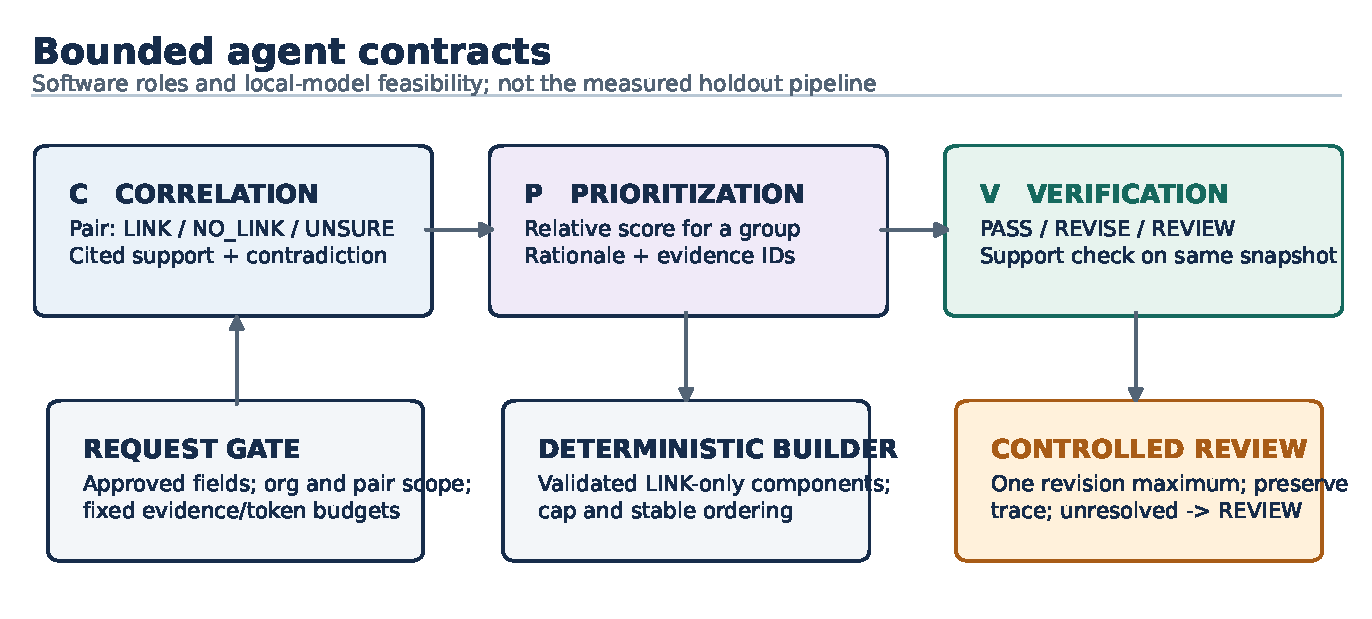
\includegraphics[width=.82\textwidth]{figures/agent_contracts.pdf}
\caption{Bounded C/P/V role contracts. The request gate restricts fields, candidate scope, evidence and budgets; C proposes links, the component builder forms groups, P assigns relative scores, and V checks cited claims. The revision branch is capped at one attempt; unresolved cases enter human review. This depicts implemented orchestration and a local prototype, not the deterministic holdout predictor or evidence of LLM superiority.}\label{fig:agentflow}\end{figure*}

\subsection{What was executed and what remains unmeasured}
The offline adapter is deliberately deterministic: it tests schema validation and control flow without an external provider. A synthetic role run recorded four candidate pairs, four components, ten role calls, one revision and one review route; its configured 2,500-token figure is an estimate, not measured model tokenization. Thirty-four synthetic assertions exercised link/no-link/unsure, citation integrity, label leakage, malformed JSON, source scope, component caps, and replay. A separate 59-assertion evaluator fixture checked pair and group metrics, ranking boundaries, and statistical procedures. Neither fixture establishes empirical SOC accuracy.

A bounded local \texttt{qwen2.5:3b} prototype exercised C/P/V on 20 organizations using local Ollama. Its candidate policy and scope differ from the full-queue statistical reference; no matched, budget-equal, fresh-label superiority test was completed. Stage-3 B0 rules and B1 BM25 have synthetic interfaces; B2 single-call and B3 three-call repeated single-LLM controls use offline stubs. These controls are important experimental designs, but their stub outputs are not empirical model baselines. A future fair comparison must freeze the same approved evidence, query set, candidate universe, abstention rules and actual model/token budget for every arm before an untouched evaluation.
